\begin{figure}[h!]
    \centering
    \caption[Effects of \emph{Plan Cuadrante} on Police Effectiveness Using Alternative Estimators]{Effects of \emph{Plan Cuadrante} on Police Effectiveness Using Alternative Estimators}
    \label{fig:figureA2_alterestim}
    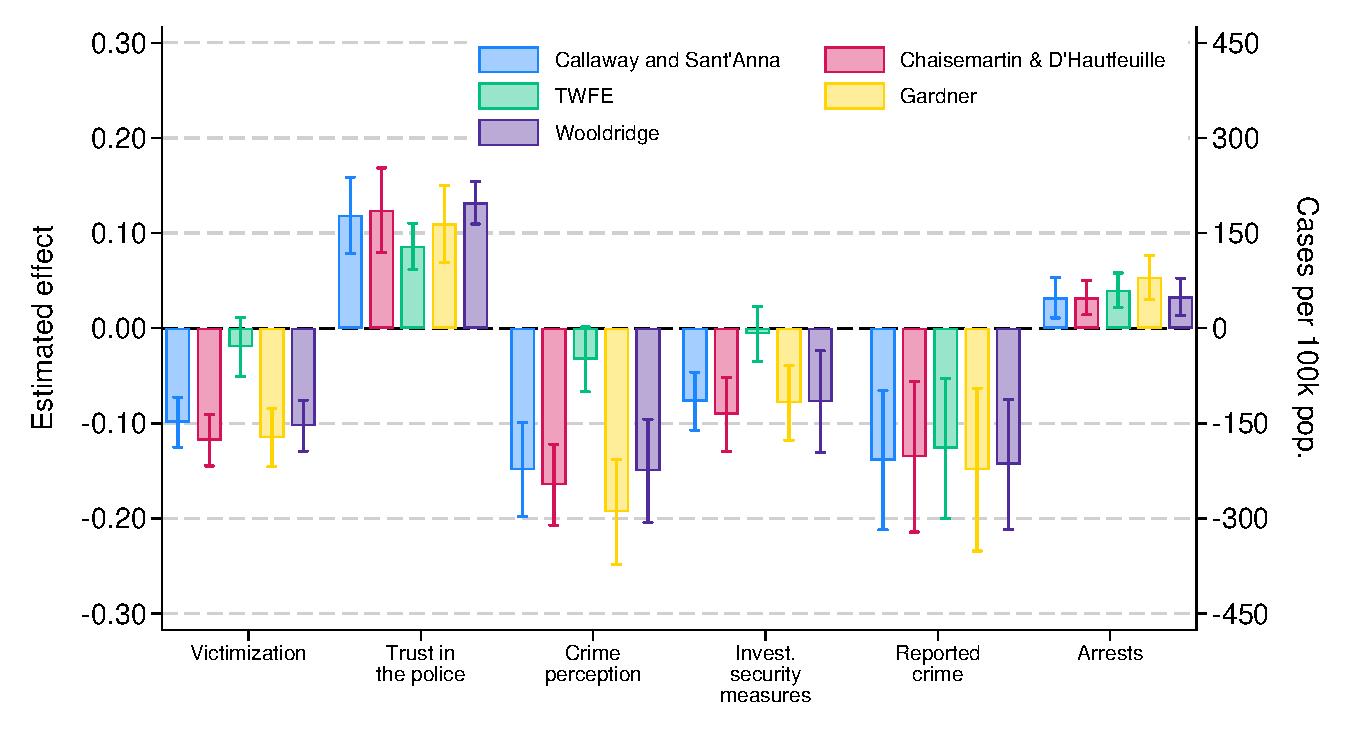
\includegraphics[width=\textwidth]{../manuscript/Graphs/Comparison_estimators_combined.pdf}
    \\[8pt]
    \begin{minipage}{0.99\textwidth}
    \footnotesize Notes: The figure reports the effects of \emph{Plan Cuadrante} on different measures of police effectiveness using various difference-in-differences estimators, including the methods developed in \citet{Callaway}, \citet{Chaisemartin}, \citet{Gardner}, \citet{wooldridge2023simple}, and the canonical two-way fixed effects (TWFE). Bars are the estimated post-treatment effects and the whiskers the 95\% confidence intervals; standard errors are clustered at the municipality level. Victimization is the probability of household victimization in the last 12 months; reported crime is the number of crimes reported to the police in the municipality per 100,000 inhabitants; crime perception is the probability of perceiving an increase in crime; investment in security measures is the probability of adopting security measures in the last twelve months; trust in the police is the probability of reporting high trust in the police; and arrests is the number of arrests per 100,000 inhabitants. Reported crime and arrests (administrative data) are read on the right axis; all other outcomes, from the ENUSC survey, are read on the left axis.
    \end{minipage}
\end{figure}
